\documentclass[conference]{IEEEtran}
\usepackage[utf8]{inputenc}
\usepackage[T1]{fontenc}
\usepackage[final]{pdfpages}
\usepackage[french]{babel}
\usepackage{colortbl}
\usepackage[table]{xcolor}
\usepackage{verbatim} 
\usepackage{graphicx}
\usepackage{algorithmicx}
\usepackage{algorithm}
\usepackage{cite}
\usepackage[caption=false,font=footnotesize]{subfig}
\usepackage[left = 3.5cm, right = 3.5cm, top = 4cm, bottom = 4cm]{geometry}

\usepackage{fancyhdr}

\title{Vérification des propriétés de sûreté d'un protocole de loterie Bitcoin}
\author{\IEEEauthorblockN{Guillaume Stunault}
\IEEEauthorblockA{Etudiant \\ Telecom Nancy}
\and \IEEEauthorblockN{Lucas Vignali} 
\IEEEauthorblockA{Etudiant \\ Telecom Nancy}
\and 
\IEEEauthorblockN{Jannik Dreier}
\IEEEauthorblockA{Maître de Conférences\\ Université de Lorraine\\ Enseignant \\ Telecom Nancy \\ Chercheur équipe PESTO \\ LORIA} 
\and \IEEEauthorblockN{Steve Kremer}
\IEEEauthorblockA{Chercheur équipe PESTO \\ LORIA} }

\date{\today}

\begin{document}

\maketitle
\begin{abstract}
Les Smart Contracts sont des programmes qui exécutent de façon automatique les termes d'un contrat, et sans besoin d'une tierce-personne de confiance pour vérifier leur bon déroulement.\cite{ethercontract}
Ils sont de plus en plus utilisés avec l'essor de la blockchain et des cryptomonnaies. Ainsi leur sécurité et leur exactitude sont cruciales pour garantir l'équité entre les différentes parties.\cite{bcfr-smart, smartdeloitte}
Nous nous sommes donc intéressés à un protocole de loterie Bitcoin \cite{955} afin de vérifier plusieurs de ces propriétés cryptographiques avec Tamarin\cite{tamarin}.
\end{abstract}
\section{Introduction}

Pour notre projet de PIDR nous avions comme sujet : \textbf{Vérification des « smart contracts » sur la blockchain}. Ce sujet nous a été proposé par M. Jannik DREIER, membre du LORIA et de l'équipe PESTO, accompagné de M. Steve Kremer. Suite à l'essor des applications liées à la blockchain et principalement celle du Bitcoin, des règles de sécurité comme les "Smart Contracts" doivent être mises en oeuvre pour la sûreté de ces protocoles.  Pour une loterie, il faut s'assurer qu'aucun participant ayant signé le contrat ne se retrouve sans paiement car l'exécution du contrat est automatique. Le but de ce PIDR a donc été de modéliser un système de smart contract. Pour cela nous avons utilisé un logiciel créé par l'équipe PESTO du LORIA : \textbf{Tamarin}\cite{tamarin}. Sur ce logiciel nous avons modélisé un protocole de loterie et vérifié certaines propriétés de sûreté (qu'une exécution incorrecte est impossible).

\section{État de l'art}
\subsection{La Blockchain}
La blockchain est une technologie de stockage et de transmission d’informations, transparente, sécurisée, et fonctionnant sans organe central de contrôle.

Par extension, une blockchain constitue une base de données qui contient l’historique de tous les échanges effectués entre ses utilisateurs depuis sa création. Ces échanges sont enregistrés sous forme de blocs, qui mis bout à bout forment une chaîne, d'où le terme blockchain. Cette base de données est sécurisée et distribuée : elle est partagée par ses différents utilisateurs, sans intermédiaire, ce qui permet à chacun de vérifier la validité de la chaîne. \cite{bcfr} \\
\begin{figure}
    \centering
    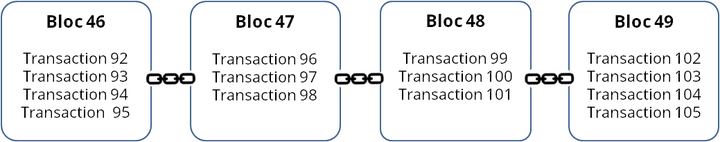
\includegraphics[scale=0.55]{blck-schema.png}
    \caption{Représentation d'une blockchain}
    \label{fig:blockchain}
\end{figure}

L’intérêt de la blockchain réside dans l’aspect décentralisé de la base de données qui est stockée sur les différents serveurs des utilisateurs et fonctionne sans intermédiaire ce qui limite les frais d’infrastructure. Cette base de données que beaucoup comparent à un grand livre comptable – public et partagé – contient un historique infalsifiable des transactions qui est mis à jour en temps réel par les utilisateurs. Les utilisateurs valident chaque transaction et vérifient la cohérence de celle-ci grâce au registre. \\

\textbf{Pourquoi infalsifiable ? } \\
Distribuée, et non centralisée, la base de données est aussi doublement sécurisée. D'abord par un système de cryptographie dite "asymétrique". Cela signifie simplement qu'il faut deux clés différentes (une privée, une publique) pour soumettre une transaction dans la blockchain. Ensuite, Chaque bloc est validé par les noeuds du réseau appelés les “mineurs”. Les "mineurs" chargés de vérifier la validité des transactions bloc par bloc sont des particuliers, rémunérés pour mettre à disposition la puissance de calcul de leurs processeurs en résolvant des fonctions de hachage cryptographique. Dans la blockchain du Bitcoin, cette technique s'appelle le "Proof-of-Work" (preuve de travail). \cite{7x7} \\
Ainsi pour manipuler la blockchain, il faudrait pouvoir falsifier plus de la moité des noeuds du système, ce qui correspond à pirater des milliers d'utilisateurs au même moment. Techniquement, il s’agit d’une prouesse impossible. \\
\begin{subfigure}
    \centering
    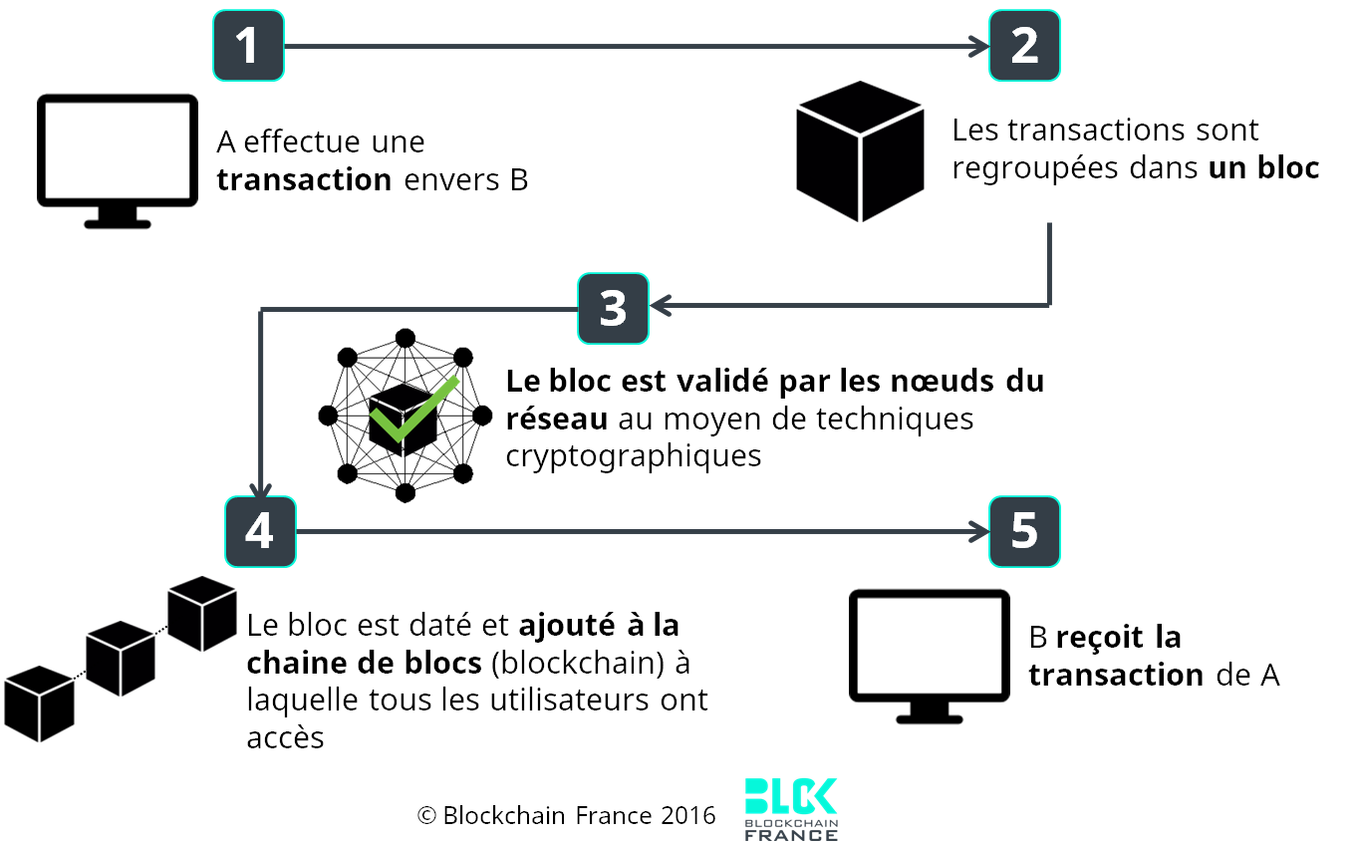
\includegraphics[scale=0.3]{blck-fonctionnement.png}
    \caption{Fonctionnement de la blockchain}
    \label{fig:blck-fonctionnement}
\end{subfigure}
\vspace{0.3cm}\\
\textbf{Le potentiel de la blockchain} \cite{bcfr}\\

Bien que souvent associé au Bitcoin et autres cryptomonnaies, le caractère décentralisé de la blockchain, couplé avec sa sécurité et sa transparence, promet des applications bien plus larges : 
\begin{itemize}
    \item Les applications pour le transfert d’actifs (utilisation monétaire, mais pas uniquement : titres, votes, actions, obligations…)
    \item Les applications de la blockchain en tant que registre : elle assure ainsi une meilleure traçabilité des produits et des actifs.
    \item Les smart contracts : il s’agit de programmes autonomes qui exécutent automatiquement les conditions et termes d’un contrat, sans nécessiter d’intervention humaine une fois démarrés. 
\end{itemize} 

\newpage

\subsection{Le Bitcoin}

Le Bitcoin est une monnaie virtuelle mais aussi un système de paiement pair à pair. C'est la première monnaie électronique décentralisé. Ce type de monnaie possède différent avantages : 
\begin{itemize}
    \item Échange de particulier à particulier ce qui implique des frais inférieurs aux banques
    \item Utilisable dans tous les pays
    \item Les comptes ne peuvent pas être gelés
    \item Pas de condition
\end{itemize}

Les bitcoins peuvent être générés par toute personne possédant un ordinateur et faisant tourner un logiciel appelé "mineur de bitcoin". Cette création de bitcoin requiert de de travailler sur chaque bloc de transaction. Ceci est ajusté par le réseau pour que la création des bitcoin soit prédictible et limitée. Enfin les bitcoin sont stockés dans des porte-monnaie électroniques. Chaque transaction est vérifiée puis stockée sur le réseau.

\subsection{Les smart contracts}
Les \textbf{smarts contracts} sont des programmes autonomes qui une fois lancés exécutent automatiquement des conditions définies préalablement et inscrites sur la blockchain. Par exemple c'est ce qu'il se passe lorsque l'on se souscrit à une assurance et que en cas de problème on est remboursé sans avoir à faire quelque chose.
L'avantage de ce type de contract repose sur le fait qu'ils sont dans la blockchain, et donc qu'il ne sont pas modifiables. Dans le cas où ils ne seraient pas dans la blockchain, alors ils seraient modifiables.

\subsection{Notions cryptographiques nécessaires à la compréhension du protocole}

\subsubsection{Cryptographie asymétrique}
Le principe de chiffrement asymétrique (appelé aussi chiffrement à clés publiques) est apparu en 1976, avec la publication d'un ouvrage sur la cryptographie par Whitfield Diffie et Martin Hellman. \cite{ccmasym, clepub}


Dans un cryptosystème asymétrique (ou cryptosystème à clés publiques), les clés existent par paires (le terme de bi-clés est généralement employé) :
\begin{itemize}
    \item Une clé publique pour le chiffrement
     \item Une clé secrète pour le déchiffrement
\end{itemize}
    
Ainsi, dans un système de chiffrement à clé publique, les utilisateurs choisissent une clé aléatoire qu'ils sont seuls à connaître (il s'agit de la clé privée). A partir de cette clé, ils déduisent chacun automatiquement une clé publique. Les utilisateurs peuvent s'échanger cette clé publique au travers d'un canal non sécurisé.

Lorsqu'un utilisateur désire envoyer un message à un autre utilisateur, il lui suffit de chiffrer le message à envoyer au moyen de la clé publique du destinataire. Ce dernier sera en mesure de déchiffrer le message à l'aide de sa clé privée (qu'il est le seul à connaître). \cite{ccmasym}
\begin{subfigure}
    \centering
    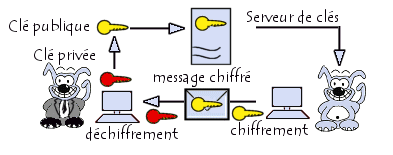
\includegraphics[scale=0.7]{asym.PNG}
    \caption{Envoi de messages par chiffrement asymétrique}
    \label{fig:asym}
\end{subfigure}

\vspace{0.3cm}
Ce chiffrement permet de s'assurer de \textbf{l'authenticité de l'expéditeur}. \cite{wikiasym}\\
\subsubsection{Les fonctions de hachage cryptographique}
Une fonction de hachage cryptographique est une fonction qui, à une donnée de taille arbitraire, associe une image de taille fixe. Une propriété essentielle est qu'elle est pratiquement impossible à inverser, c'est-à-dire que si l'image d'une donnée par la fonction se calcule très efficacement, le calcul inverse d'une donnée d'entrée ayant pour image une certaine valeur se révèle impossible sur le plan pratique. Pour cette raison, on dit d'une telle fonction qu'elle est à sens unique.\cite{wikihash, ryxhash}. Les fonctions de hachage sont utilisées pour garantir \textbf{l'intégrité} d'une donnée. Si un message est corrompu, son haché ne sera plus le même. \cite{igmsign}\\
Comme une fonction de hachage transforme un message de taille arbitraire en message de taille fixe. Il y a donc un problème : comme il y a plus de messages possibles que de hachés possibles, plusieurs messages peuvent donc avoir le même haché. Cela s'appelle une collision. \cite{ryxhash, cryptohash}\\
Pour une fonction de hachage F, on demande qu'elle soit :
\begin{itemize}
    \item résistante au calcul de préimage (étant donné y difficile de trouver y = F(x))
    \item résistante au calcul de seconde préimage (étant donné x, difficile de trouver x', tel que F(x) = F(x'))
    \item résistante aux collisions (difficile de trouver x et x', tel que F(x) = F(x'))
\end{itemize}
Il est aujourd'hui très difficile de trouver des collisions sur les fonctions de hachage actuelles (SHA2-SHA3). \\
Les fonctions de hachage dans Tamarin sont résistantes aux 3 propriétés ci-dessus. \\

\subsubsection{Signature}
La signature d'un document utilise à la fois la cryptographie asymétrique et les fonctions de hachage. C'est en effet par l'association de ces deux techniques que nous pouvons obtenir les 5 caractéristiques d'une signature (authentique, infalsifiable, non réutilisable, inaltérable, irrévocable). \cite{igmsign}

Si Alice souhaite signer un document et l'envoyer à Bob : \\
    Tout d'abord, elle génére \textbf{l'empreinte} du document au moyen d'une fonction de hachage.\\
    Puis, elle crypte cette empreinte avec sa clé privée.

    Elle obtient ainsi la signature de son document. Elle envoie donc ces deux éléments à Bob

    Pour vérifier la validité du document, Bob doit tout d'abord déchiffrer la signature en utilisant la clé publique d'Alice. Si cela ne fonctionne pas, c'est que le document n'a pas été envoyé par Alice.\\
    Ensuite, Bob génère l'empreinte du document qu'il a reçu, en utilisant la même fonction de hachage qu'Alice (On supposera qu'ils suivent un protocole établi au préalable).\\
    Puis, il compare l'empreinte générée et celle issue de la signature.

    Si les deux empreintes sont identiques, la signature est validée. Nous sommes donc sûr que : \\
        C'est Alice qui a envoyé le document, \\
        Le document n'a pas été modifié depuis qu'Alice l'a signé.
\cite{igmsign}
\subsection{Tamarin}

\section{Le protocole de loterie}
Nous allons analysé ce protocole de smart contract qui implémente une loterie Bitcoin. \cite{955}
Ce protocole garantit :
\begin{itemize}
\item chaque joueur honnête aura (en moyenne) un gain non négatif, même dans la
présence d'adversaires qui jouent contre 
\item Si tous les joueurs sont honnêtes, le protocole simule une loterie ordinaire : 1 joueur remporte les mises des autres joueurs 
\end{itemize}
Le protocole utilise un arbre de tournoi : chaque manche le gagnant remporte la mise de l'adversaire \\
\\ \\
\begin{subfigure}
    \centering
    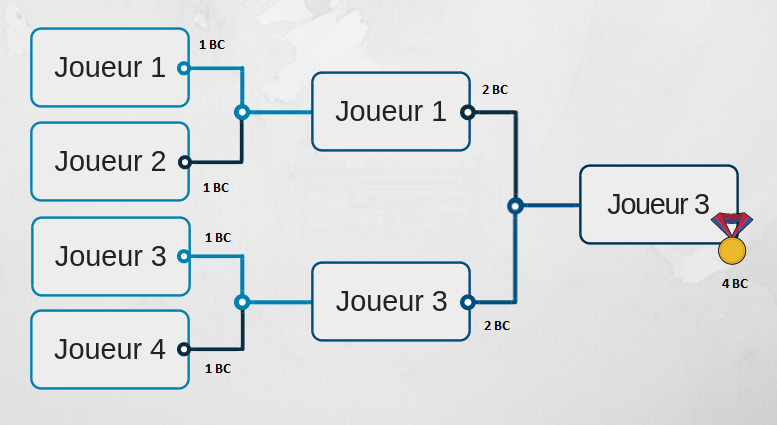
\includegraphics[scale=0.4]{arbre-tournoi.png}
    \caption{Protocole pour 4 joueurs avec mise de départ : 1 Bitcoin}
    \label{fig:my_label}
\end{subfigure}
\vspace{0.3cm}\\
Initialisation : \\
\begin{itemize}
\item chaque joueur génère N paires de clés, O(N\up{2}) signatures (N signatures pour N paires de clé * N transactions Win, Timeout... pour chaque joueur) et log(N) secrets qu'il hash ensuite pour tous les matchs qu'il va jouer.
\item on vérifie que les hashs ne sont pas réutilisés
\item ensuite il pose la mise en signant une transaction Init
\item si un joueur ne pose pas la mise, les autres récupèrent leur mise
\item Init est ajouté à la blockchain
\item La transaction doit s'effectuer dans un temps donné, assez long pour qu'il permette la transaction. Ce temps est calculé pour permettre la géneration des clés 
\item Init est ensuite séparée en N mises de départ : Win(p,p) ajoutées à la blockchain \\
\end{itemize}
\\

Execution :  \\
\begin{itemize}
\item C'est la phase de match, soient $\pi_{k}$ le match actuel, $p_{1}$ et $p_{2}$ les joueurs qui s'affrontent
\item Au départ, on ajoute à la blockchain, les transactions Win( $\pi_{k-1}$, $p_{1}$) et Win( $\pi_{k-1}$, $p_{2}$) si ça n'a pas déjà été fait
\item $p_{1}$ commence, on ajoute Turn1($\pi_{k}$, $p_{1}$, $p_{2}$) à la blockchain :  $p_{1}$ doit donc révéler son secret à temps en l'ajoutant, comme in-scipt dans Turn2($\pi_{k}$, $p_{1}$, $p_{2}$)
\item Ainsi, $p_{2}$ peut vérifier que le hash de $p_{1}$ correspond au hash envoyé au départ
\item $p_{2}$ connait son propre secret et exécute la fonction aléatoire w = winner($\pi_{k}$, $p_{1}$, $p_{2}$, $Sk_{1}$, $Sk_{2}$)
\item $p_{2}$ ajoute finalement à la blockchain la transaction Win(w, $\pi_{k}$) avec pour in-script son secret $Sk_{2}$.
\item Chaque joueur doit chacun son tour réveler sa clé dans un temps imparti sinon il perd. \\
\end{itemize}
\\
Mise : \\
 A tous les tours, chaque joueur mise 1 bitcoin. Pour éviter la fraude et qu'un joueur quitte la partie en plein milieu avec l'argent qu'il a récolté, chaque joueur pose au début une somme de bitcoins égale au nombre de parties possibles par un joueur. Ainsi à chaque partie gagné un bitcoin est retiré de cette somme, et si le joueur quitte la partie en plein milieu cette est reversé à chaque joueur affronté précédemment ce qui fait que le joueur en question ne gagne pas d'argent. Dans le cas ou il perd une manche cette mise lui est rendu.

\section{Protocole réalisé}
Nous avons simplifié le protocole au maximum pour tester ses divers propriétés de sécurité. \\
Nous prenons désormais uniquement 2 joueurs A et B, et une seule manche de match. \\
La mise vaut pour le moment : 1 bitcoin \\
De plus, pour modéliser la blockchain, nous considérons les traces de Tamarin. En effet, la blockchain rend les transactions enregistrées consultables à chaque moment tout comme les traces de Tamarin.


\begin{itemize}
    \item A et B génèrent chacun une clé publique et une clé secrète
    \item A partir de cette clé secrète, le protocole assigne un porte-monnaie avec 3 bitcoins à chaque joueur
    \item Chacun des 2 joueurs génère ensuite un secret pour le match, et envoie son hash signé sur le réseau.
    \item La blockchain retire 1 Bitcoin du porte-monnaie de A et B pour créer une mise
    \item La blockchain crée un contrat où A et B posent leurs mises. Lorsque les 2 mises sont posées, le match peut commencer.
    \item La blockchain crée un contrat où A doit révéler son secret. Elle vérifie que le hash du secret envoyé correspond au hash envoyé avant le match
    \item Idem pour B
    \item Lorsque la blockchain possède les 2 hashs, elle peut déterminer aléatoirement un gagnant entre A et B.
    \item La blockchain ajoute les 2 Bitcoins au porte-monnaie du gagnant.
\end{itemize}

Normalement, la blockchain est censé déterminer un gagnant avec une fonction sur la parité des secrets (processus qui est défini aléatoire et non truquable). Pour modéliser cela sur Tamarin, nous avons crée 2 règles identiques de victoire : une avec A, une avec B. Et Tamarin choisit aléatoirement une de ces 2 règles.

\section{Propriétés à prouver}
Nous avons décidé, pour vérifier le bon fonctionnement du protocole d'implémenter des propriétés simples. Nous avons donc modéliser 3 propriétées :
\begin{itemize}
    \item Il existe une exécution normale du protocole
    \item A la fin, le porte-monnaie de l'un contient 4 bitcoins, et celui du perdant 2 bitcoins
    \item Il y a un seul gagnant à la fin, qui peut être le joueur A ou le joueur B \\
\end{itemize}
Ces propriétés étaient en partie formulée dans la documentation du protocole.
Chaque preuve de ses propriétées se décrit sous forme de lemme. Par exemple pour vérifier que le joueur A ou le joueur B peut gagner il faut regarder si il existe une version de l'exécution du protocole où à la fin on a WinnerA ou WinnerB, les fonctions définissant le gagnant.

Pour vérifier que la somme d'argent en jeu est juste pendant toute l'exécution du contrat, nous avons ajouté un fait Monnaie qui contient le porte-monnaie du joueur A, le porte-monnaie du joueur B, la somme mise en jeu et le total 

\section{Ouverture}
Pour la suite nous avons plusieurs possibilité. Nous avons modéliser des propriétées simples pour nous permettre de vérifier le bon déroulement du protocole. Cependant il y a plusieurs modification que l'on pourrait faire. Tout d'abord, nous avons modéliser le protocole avec seulement 2 joueurs, le but étant de le modéliser pour N joueurs. Dans ce protocole nous avons aussi défini deux règles WinnerA et WinnerB définissant le gagnant, A ou B. Ces règles ne correspondent pas exactement à celle explicité dans le protocole de départ. En effet dans la documentation du protocole il est expliqué que le gagnant est définie à partir de la parité des secrets. Ce type de règle étant difficilement implémentable en Tamarin, nous avons décidé de réaliser une règle plus simple qui choisi A ou B comme gagnant

Nous aurions pû également nous intéresser à vérifier des propriétés de \textit{liveness} (la propriété sera vraie après une certaine étape de l'exécution) \cite{vivacite}.
Par exemple, garantir qu'un joueur qui quitte la partie ne récupérera son argent qu'avant Init.


\section{Conclusion}

\section{Remerciements}






\begin{comment}
 N = 2^(L) joueurs
 2^(L)-1 = N-1 1v1 joués
 pi = numéro du match
\end{comment}


\newpage
\bibliographystyle{plain-fr}
\bibliography{bibliography.bib}


\newpage
\begin{tabular}{|m{3cm}|m{7cm}}
\hline
\rowcolor{grey!40} \textbf{Date} & \textbf{Travail effectué}  \\ 
\hline 
\rowcolor{grey!10}  07/02/2018 & Découverte du sujet \\
\hline
\rowcolor{grey!10}  14/02/2018 & Installation de Tamarin \newline Choix du protocole : loterie \\
\hline
\rowcolor{grey!10}  15/03/2018 & Compréhension du sujet \newline Rédaction du rapport \newline Découverte Tamarin \\
\hline
\rowcolor{grey!10}  04/04/2018 & Première version compilable du protocole \\
\end{tabular}



\end{document}


